\documentclass[12pt,a4paper,openright]{scrreprt}

% DEBUG stuff
\usepackage{refcheck}

% PACKAGES + MODIFICATIONS
\usepackage[T1]{fontenc} % Use 8-bit encoding that has 256 glyphs
\usepackage[utf8]{inputenc}
\usepackage{lmodern}
\usepackage{textgreek}
\usepackage[activate={true,nocompatibility},draft,tracking=true,factor=1100,stretch=10,shrink=10]{microtype}
% activate={true,nocompatibility} - activate protrusion and expansion
% final - enable microtype; use "draft" to disable
% factor=1100 - add 10% to the protrusion amount (default is 1000)
% stretch=10, shrink=10 - reduce stretchability/shrinkability (default is 20/20)
\usepackage[english]{babel}

% math
\usepackage{amsmath}
\usepackage{amssymb}
\usepackage{amsfonts}
\usepackage{mathtools}
\usepackage{tensor}
\usepackage{commath}
\usepackage{bm} % bold in math mode
\usepackage{units}

%layout and style
\usepackage[hmarginratio=1:1,top=32mm,columnsep=20pt]{geometry} % Document margins
\setlength{\parindent}{0pt}  % no indendation for new paragraphs

\usepackage[automark,headsepline]{scrlayer-scrpage} %headings
\pagestyle{scrheadings}
% \ihead{Benjamin Rottler}
% \chead{Term Paper}
% \ohead{August 2016}
% \ofoot{\pagemark}
% \cfoot{}

%graphics
\usepackage{graphicx}

% floats, figures tables
\usepackage{float}
\usepackage{booktabs}   % tables for publications
\usepackage[labelfont=bf]{caption} % bold captions

%hyperref
\newcommand{\hreftitle}{Master thesis} % TODO set right title
\newcommand{\hrefauthor}{Benjamin Rottler}
\usepackage[pdftex]{hyperref}
\hypersetup{%
    pdftitle={\hreftitle},
    pdfsubject={\hreftitle},
    pdfkeywords={},  % TODO
    pdfauthor={\hrefauthor},
    pdfcreator={\hrefauthor},
    pdfproducer={\hrefauthor},
    bookmarksnumbered=true, % bookmarks are numbered
    bookmarksopen=true,     % show bookmarks at start of pdf viewer
    bookmarksopenlevel=2,   % level to which the bookmarks are opened
    bookmarksdepth=3,       % depth of bookmarks
    unicode=true,           % non-Latin characters in pdf viewer's bookmarks
    pdftoolbar=false,       % show pdf viewer's toolbar?
    pdfmenubar=true,        % show pdf viewer's menu?
    pdffitwindow=false,     % window fit to page when opened
    pdfstartview={FitH},    % fits the width of the page to the window
    pdfnewwindow=true,      % links in new window
    pdfborder={0 0 1},		% no border for links
    colorlinks=false,		% false: black links; true: colored links
    linkcolor=red,          % color of internal links (change box color with
    % linkbordercolor)
    citecolor=green,        % color of links to bibliography
    filecolor=magenta,      % color of file links
    urlcolor=blue			% color of external links
}
\usepackage[nottoc,numbib]{tocbibind} % put references in TOC

% other packages
\usepackage{cite} % improved citation handling
\usepackage[capitalise]{cleveref}  % clever references

%----------------------------------------------------------------------------------------
%	Glossary
%----------------------------------------------------------------------------------------
\usepackage[xindy]{glossaries}
\makeglossaries%
\usepackage[xindy]{imakeidx}
\makeindex%

\newacronym{HEP}{HEP}{high-energy physics}
\newacronym{ML}{ML}{machine learning}
\newacronym{DT}{DT}{decision tree}
\newacronym{BDT}{BDT}{Boosted Decision Tree}
\newacronym{NN}{NN}{Neural Network}

\newcommand{\hep}{\gls{HEP}}
\newcommand{\ml}{\gls{ML}}
\newcommand{\bdt}{\gls{BDT}}
\newcommand{\bdts}{\glspl{BDT}}
\newcommand{\nn}{\gls{NN}}
\newcommand{\nns}{\glspl{NN}}


%----------------------------------------------------------------------------------------
%	NEW COMMANDS
%----------------------------------------------------------------------------------------

% \let\originalleft\left  %fix bracket spacing when using \left( \right)
% \let\originalright\right
% \renewcommand{\left}{\mathopen{}\mathclose\bgroup\originalleft}
% \renewcommand{\right}{\aftergroup\egroup\originalright}

% math
\renewcommand{\abs}[1]{\ensuremath{\left|#1\right|}}
\renewcommand{\vec}{\mathbf}

% variables
\newcommand{\pt}{\ensuremath{p_\text{T}}}
\newcommand{\et}{\ensuremath{E_\text{T}}}
\newcommand{\etmiss}{\ensuremath{E_\text{T}^\text{miss}}}
\newcommand{\dr}{\ensuremath{\Delta R}}
\newcommand{\drll}{\ensuremath{\Delta R (\ell\ell)}}

% particles
\newcommand{\Z}{\ensuremath{Z}}
\newcommand{\JPsi}{\ensuremath{J/\Psi}}
\newcommand{\epem}{\ensuremath{e^+e^-}}

\begin{document}

\tableofcontents

\chapter{Introduction}\label{cha:introduction}

In elementary particle physics the fundamental constituents of nature and their interactions are studied.
In the 1960s and 1970s the Standard Model (SM) of particle physics was developed to provide an accurate description of all elementary particles which are known today
and their fundamental interactions.
The particles can be classified based on their spin: \emph{fermions} have a half-integer spin and \emph{bosons} have an integer spin.
Three out of the four fundamental interactions, the electromagnetic, strong, and weak interaction, are incorporated in the SM as
relativistic quantum field theories.
No formulation of gravity as a relativistic quantum field theory is found yet.
However, the influence of gravity at the energy scales considered in particle physics is minor and therefore can be neglected.

With the help of the Standard Model it was possible to predict several particles, which were later found in nature,
for example the massive $W^\pm$- and $Z^0$-bosons which were first observed in 1983~\cite{ZDiscovery,WDiscovery,ZeeDiscovery,WeDiscovery}.
In earlier formulations of the SM no mass terms for fermions and bosons were included, which stands in contrast to measurements of fermion and boson masses.
For example, the $W^\pm$- and $Z^0$-bosons have a mass of $m_{W^\pm} = \SI{80.4}{\GeV}$ and $m_{Z^0} = \SI{91.2}{\GeV}$, respectively~\cite{PDG}.
This conflict was solved by the introduction of the
Englert--Brout--Higgs--Guralnik--Hagen--Kibble mechanism~\cite{HiggsMecha1,HiggsMecha2,HiggsMecha3,HiggsMecha4,HiggsMecha5,HiggsMecha6} (short: Higgs mechanism)
which uses the principle of spontaneous symmetry breaking.
A new scalar field, the Higgs field, is introduced.
The interaction of fermions and bosons with vacuum expectation value of the Higgs field leads to required mass terms of the particles.
The particle associated with the Higgs field is the \emph{Higgs boson}, which was however, at that time, not yet observed.
During the last decades great effort was put into the search for the Higgs boson at different collider experiments, until it
was found with the ATLAS\footnote{\textbf{A} \textbf{T}oroidal \textbf{L}HC \textbf{A}pparatu\textbf{S}} and
CMS\footnote{\textbf{C}ompact \textbf{M}uon \textbf{S}olenoid} experiments at
CERN\footnote{\textbf{C}onseil \textbf{E}uropéen pour la \textbf{R}echerche \textbf{N}ucléaire} in 2012~\cite{HiggsDiscoveryATLAS,HiggsDiscoveryCMS}.
The mass of the newly found particle was determined to be $m_H = (125.09 \pm 0.21 \text{(stat.)} \pm 0.11 \text{(sys.)})\,\text{GeV}$
in a combined measurement of the ATLAS and CMS collaboration~\cite{MassCombinedMeas}.
After the Higgs boson was found at CERN, Peter Higgs and Francois Englert were awarded the Nobel Prize in 2015 for the formulation of
the underlying theory.

The $H \to \tau\tau$ decay mode is an important decay channel of the Higgs boson, since it it provides the most sensitive measurement
of the Yukawa couplings of the Higgs boson.
Additional, the $H \to \tau\tau$ decay channel can be used to probe a potential CP mixing and lepton-flavour violating decays of the Higgs boson.
During the first data-taking period at the LHC in 2011 and 2012 evidence for this decay channel was found at the ATLAS experiment with
a sensitive of $4.5\sigma$~\cite{HTauTauRun1}.
Due to limited statistic the observation where a sensitivity of $5\sigma$ is required could not be made.

In this thesis the $\Httllfull$ decay channel is considered, where both leptons decay Leptonically, with the
combined 2015 and 2016 dataset of the second data-taking period corresponding to an integrated luminosity of $\lumi = \SI{36.1}{\invfb}$
at a center-of-mass energy of $\sqrt{s} = \SI{13}{\TeV}$.
A method is developed to increase the sensitivity in this decay channel with the help of multivariate techniques.
More precisely, the usage of boosted decision trees (BDTs), a machine-learning algorithm, is investigated.

This thesis is structured as follows.
First the Standard Model is introduced and an overview of the current status of Higgs-boson property measurements is given in \cref{cha:theory}.
In \cref{cha:setup} the LHC and ATLAS experiment are described.
The signal and background processes considered in the analysis of $\Httllfull$ are discussed in \cref{cha:processes}, followed by an overview
of the reconstruction of physical objects in \cref{cha:object_selection}.
The event selection is described in \cref{cha:event_selection} and the strategy to estimate specific backgrounds
is presented in \cref{cha:background_estimation}.
An overview of the theoretical aspects of BDTs is given in \cref{cha:bdt} and their application to the analysis of the $\Httllfull$ process
is discussed in \cref{cha:mva}.
In \cref{cha:systematics} the systematic uncertainties are presented.
The thesis closes with a description of the statistical procedure and a discussion of the results in \cref{cha:fit}, followed
by a summary of the analysis and an outlook for further studies in \cref{cha:conclusion}.

\chapter{Theory}\label{cha:theory}

This chapter introduced the theoretical background on which this analysis is based on.
First, the Standard Model (SM) of particle physics, which describes the fundamental particles and their interactions, is discussed.
Then an overview of the phenomenology of hadron scattering is given.
Afterwards the Higgs-boson production and decay is discussed in detail and past measurements of the Higgs boson are presented.

\section{The Standard Model of Particle Physics}\label{sec:theory:sm}

The Standard Model of particle physics was developed during the 1960s and 1970s and
describes elementary particles and their fundamental interactions to great precision.
It is a relativistic quantum field theory based on the principle of local gauge symmetries.
Several particles like the $W^\pm$- and $Z^0$- bosons and the top-quark were predicted by the SM and later discovered in
nature~\cite{ZDiscovery,WDiscovery,TopDiscovery,ZeeDiscovery,WeDiscovery,TopDiscoveryD0}.
Out of the four fundamental forces it describes only three, it was not yet successful to combine the
formulation of gravity with the other interactions.
But because gravity has only a minor effect on particles at the energy scales accessible at current collider experiments
it can be neglected.

The contents of this section are based on~\cite{Griffiths,HalsenMartin,PeskinSchroeder} if not noted otherwise.

\subsection{Elementary Particles}\label{sub:theory:particles}

The elementary particles of the SM can be divided into fermions which carry half integer spin and bosons with a full integer spin.
Fermions can further be split into leptons which only interact via the electroweak force and quarks which interact via
both the electroweak and strong force.
Empirical evidence shows that there are three generations of both leptons and quarks.
This cannot be predicted by the SM, it was rather used as input.
The three generations are copies of each other which are identical expect for the flavour and mass of the particles.
They are sorted in ascending order by the masses of the particles..
There exist two elementary particles for each flavour.

In the case of leptons there is the electron ($e$), muon ($\mu$), and tau lepton ($\tau$) which all have a
charge\footnote{The electric charge is given in units of the fundamental electric charge $q_e = \SI{1.602e-19}{\coulomb}$~\cite{PDG}.} of $Q = -1$.
Each lepton is associated with a neutral particle called the neutrino ($\nu_e$, $\nu_\mu$, $\nu_\tau$).

For quarks one particle of each flavour has a charge of $Q = \frac{2}{3}$. These particles are called the up-, charm-, and
top-quark.
The other quarks are the down-, strange-, and bottom-quark with charge of $Q = -\frac{1}{3}$.
An overview of the fermions in the SM with their charges and approximate masses is given in \cref{tab:theory:fermions}.

Each particle has its corresponding anti-particle, which has the same quantum numbers up to charge and magnetic momentum properties.

Most matter surrounding us consists only of fermions from the first generation, namely the up- and down-quark which form protons and neutrons and the electron.
All other particles are only accessible via cosmic radiation or collider experiments.

\begin{table}[htpb]
    \centering
    \caption{Overview of the fermions in the Standard Model~\cite{PDG}.}\label{tab:theory:fermions}
    \begin{tabular}{lcclcl}
        \toprule
                                 & Generation               & \multicolumn{2}{l}{Flavour}           & Charge [$q_e$] & Mass [GeV] \\  \midrule
        \multirow{6}{*}{Leptons} & \multirow{2}{*}{\nth{1}} & $e$        & Electron                 & $-1$    & $\approx \num{0.5e-3}$ \\
                                 &                          & $\nu_e$    & Electron neutrino        & $ 0$    & $ < \num{2e-9}$        \\ \cmidrule{2-6}
                                 & \multirow{2}{*}{\nth{2}} & $\mu$      & Muon                     & $-1$    & $\approx \num{106e-3}$ \\
                                 &                          & $\nu_\mu$  & Muon Neutrino            & $ 0$    & $ < \num{0.19e-3}$ \\ \cmidrule{2-6}
                                 & \multirow{2}{*}{\nth{3}} & $\tau$     & $\tau$-lepton            & $-1$    & $\approx \num{1.777}$ \\
                                 &                          & $\nu_\tau$ & $\tau$-lepton neutrino   & $ 0$    & $ < \num{18e-3}$ \\ \midrule
        \multirow{6}{*}{Quarks}  & \multirow{2}{*}{\nth{1}} & $u$        & Up                       & $ \frac{2}{3}$ & $\approx \num{2.2e-3}$ \\
                                 &                          & $d$        & Down                     & $-\frac{1}{3}$ & $\approx \num{4.7e-3}$ \\ \cmidrule{2-6}
                                 & \multirow{2}{*}{\nth{2}} & $c$        & Charm                    & $ \frac{2}{3}$ & $\approx \num{1.28}$ \\
                                 &                          & $s$        & Strange                  & $-\frac{1}{3}$ & $\approx \num{96e-3}$ \\ \cmidrule{2-6}
                                 & \multirow{2}{*}{\nth{3}} & $t$        & Top                      & $ \frac{2}{3}$ & $\approx \num{173}$ \\
                                 &                          & $b$        & Bottom                   & $-\frac{1}{3}$ & $\approx \num{4.18}$ \\
        \bottomrule
    \end{tabular}
\end{table}

The fundamental interactions of the SM are mediated by gauge bosons with spin one.
An overview of the gauge bosons in the SM is given in \cref{tab:theory:bosons}.

The photon ($\gamma$) is the mediator of the electromagnetic force.
It couples to the electric charge $Q$ of the particles.
Due to the fact that the photon is massless and stable, the electromagnetic force has infinite range.

The weak interaction is transmitted via the massive $W^\pm/Z^0$-bosons, which couple to the weak isospin $I_3$ of the particles.
All fermions have a weak isospin of $I_3 = \frac{1}{2}$, the $W^\pm$-bosons have a weak isospin of $I_3 = \pm 1$ and the $Z^0$ boson
has a weak isospin of $I_3 = 0$. %TODO neutral / weak charged current, w: right handed particles, left handed anti particles
In contract to the photon the $W^\pm$- and $Z^0$-bosons are quite massive with a mass of $m_{W^\pm} = \SI{80.4}{\GeV}$ and
$m_{Z^0} = \SI{91.2}{\GeV}$, respectively~\cite{PDG}.
This leads to the weak coupling at low energies and the low range of the weak interaction.

The strong force is mediated by eight gluons ($g$), which are massless and couple to the color charge.
All quarks and gluons have a color charge.
Because the gluons have a color charge themselves, self-interaction is possible, which limits the range of the
strong force.

The Standard Model contains also one scalar spin-0 particle, the Higgs boson.
It has been detected in 2012 with the ATLAS and CMS detectors~\cite{HiggsDiscoveryATLAS,HiggsDiscoveryCMS}.
The Higgs boson and the current measurements of Higgs-boson properties are discussed in detail in \cref{sec:theory:higgs,sec:theory:measurements}.

\begin{table}[htpb]
    \centering
    \caption{Overview of the gauge bosons in the Standard Model~\cite{PDG}.}\label{tab:theory:bosons}
    \begin{tabular}{lclccc}
        \toprule
        Interaction             & \multicolumn{2}{l}{Gauge boson}   & Charge [$q_e$]    & Mass [GeV] & Distance [m] \\  \midrule
        Electromagnetic         & $\gamma$  & Photon                & $0$               & 0          & $\infty$                         \\ \cmidrule{1-6}
        \multirow{2}{*}{Weak}   & $W^\pm$   & $W^\pm$ boson         & $\pm 1$           & 80.4       & \multirow{2}{*}{$< \num{e-15}$}  \\
                                & $Z^0$     & $Z^0$ boson           & $0$               & 91.2       &                                  \\ \cmidrule{1-6}
        Strong                  & $g$       & Gluon (8x)            & $0$               & 0          & $\approx \num{e-15}$             \\
        \bottomrule
    \end{tabular}
\end{table}


\section{Hadronic scattering and parton model}\label{sec:theory:hadronscattering}

Today Higgs bosons can only be investigated at hadron colliders.
A hadron is no fundamental particles, it is a combination of several quarks bound by the strong force.
In the following a two-particle scattering
\begin{equation}
    1 + 2 \to 3 + 4
\end{equation}
is discussed.
The four-momenta of the particles are denoted by $p_i$ with $i = 1,\ldots,4$.

The structure of hadrons can be described with the structure functions $W_1(Q^2, \nu)$ and $W_2(Q^2, \nu)$,
which depend on the squared four-momentum transfer
\begin{equation}
    Q^2 = -q^2 = - (p_1 - p_3)^2
\end{equation}
and the transferred energy $\nu = E' - E$.
The structure functions are measured in deep inelastic electron--nucleon scattering experiments.
The cross-section for those scatterings can be written as~\cite{drell64, bjo:scaling}
\begin{equation}
    \frac{\dif \sigma}{\dif\Omega \dif E'} = \frac{\alpha^2}{4 E^2 \sin^4 \frac{\theta}{2}}
    \left[ W_2(Q^2, \nu) \cos^2 \frac{\theta}{2} + 2 W_1(Q^2, \nu) \sin^2 \frac{\theta}{2} \right ],
\end{equation}
with the fine-structure constant $\alpha$, the energies $E$ and $E'$ of the electron before and after the scattering,
and the scattering angle $\theta$, the angle between the electron beam, and the scattered electron.

For large energies the quantities $Q^2$ and $\nu$ are not longer independent of each other.
$W_1$ and $\nu W_2$ only depend on a single variable, the \emph{Bjorken scaling variable}, $x$:
\begin{equation}
    x = \frac{Q^2}{2 M \nu} \,,
\end{equation}
where $M$ is the mass of the nucleon.
In the asymptotic limit the structure of hadrons can be described with the structure functions $F_1(x)$ and $F_2(x)$,
\begin{equation}
    \begin{split}
        \lim_{Q^2, \nu \to \infty} W_1(Q^2, \nu) &= F_1(x) \,, \\
        \lim_{Q^2, \nu \to \infty} \nu W_2(Q^2, \nu) &= F_2(x) \,.
    \end{split}
\end{equation}
This phenomenon was discovered experimentally and is called \emph{Bjorken scaling} after its discoverer, J.\ D.\ Bjorken~\cite{bjo:scaling}.

Richard Feynman and E. A. Paschos proposed a descriptive model for the structure of the proton, the so called
\emph{parton model}~\cite{feyn69,bjo:epscattering}.
According to this model the proton can be described as an accumulation of free, charged, point-like particles, the \emph{partons}.
This view makes only sense in the \emph{infinite momentum frame}, a reference frame where the proton has infinite
momentum.\footnote{The center-of-mass frame of the colliding particle and the proton is a good approximation
for such a frame at high energies~\cite{bjo:epscattering}.}
In this frame the transverse momenta and masses of the partons are negligible.
The four-momentum $p_i$ of a parton $i$ is a fraction $x_i \ (0 \leq x_i \leq 1)$ of the total four-momentum $p$ of the proton:
\begin{equation}
    p_i = x_i p\,, \qquad\text{with } \sum_i x_i = 1\,.
\end{equation}
The fraction $x_i$ can be identified with the Bjorken scaling variable~\cite{bjo:epscattering}: $x$ is the momentum fraction of the parton
by which the lepton has been scattered.

The generalized probability density to find a parton $i$ with the longitudinal momentum fraction $x_i$ is defined as the
parton distribution function (PDF) $f_i(x, M_\text{F}^2)$.
$M_\text{F}$ is the factorization scale, a distinction between hard and soft scattering.
Since PDFs cannot be calculated within perturbation theory, they are determined with the help of fits to experimental data.
The DGLAP evolution equations (Dokshitzer, Gribov, Lipatov, Altarelli, Parisi)~\cite{dglap:d, dglap:gl, dglap:ap}
can be used to evolve the experimentally provided PDFs to other factorization scales, which may not be accessible by experiments.

\cref{fig:theory:pdfs} displays the PDFs of different partons in protons.
The PDFs of the up and down quarks are not equal to the PDFs of their antiquarks.
This is caused by the internal structure of the proton.
There are three \emph{valence quarks}, two up and one down quark, which together determine the quantum numbers of the proton.
These quarks constantly exchange gluons, which may produce a temporary quark--antiquark pair, the so-called \emph{sea quarks}.
Because the sea quarks only exists in pairs, the probability to find an up or down quark in a proton is larger than finding an
antiup or antidown quark.
\begin{figure}[htb]
    \centering
    \includegraphics[width=0.7\textwidth]{./figures/theory/nnpdf.png}
    \caption{PDFs for different partons as a function of the Bjorken scaling variable $x$
             for two different factorization scales $Q^2 = \SI{10}{\GeV\squared}$ and $Q^2 = \SI{e4}{\GeV\squared}$.
             The PDF set is NNPDF3.1 (NNLO)~\cite{nnpdf3.1}.}\label{fig:theory:pdfs}
\end{figure}
Another property of quark partons is indicated: It is less probable to find a quark with a higher mass.
The probability to find a photon is highly repressed, in contrast to the gluon PDF, which has the highest value for small $x$.

A dependency on the factorization scale $Q^2$ is recognizable.
The predicted independence of the PDFs from $Q^2$ only holds approximately for certain values.
But the parton model of Feynman still can be used as a foundation to describe inelastic scattering.
There are more complicated models like the \emph{QCD-improved parton model}~\cite{col98}, where
partons are allowed to interact between each other by exchanging gluons.

\todo{Shorten/rephrase section}

\section{The Higgs Boson}\label{sec:theory:higgs}

\subsection{Higgs Boson Production in Proton--Proton Collisions}
\label{sub:theory:higgs:production}

In proton--proton collisions at the LHC the parton model as described above can be applied.
To calculate the cross-section of the production of a particle $X$ in proton--proton collisions the
cross-section at parton level $\hat{\sigma}_{ij\to X}$ has to be weighted with the PDFs and all
possible momentum fractions need to be considered, as prescribed by the factorization theorem~\cite{DRELL1971578}.
Mathematically speaking this is a convolution of the PDFs with the partonic cross-section,
\begin{equation}
    \sigma_{ij\to X} = \int_{0}^{1} \dif x_i \int_{0}^{1} \dif x_j \,
    f_i \left( x_i \right ) f_j \left( x_j \right ) \hat{\sigma}_{ij\to X} \,.
\end{equation}
The general expression of the partonic cross-section is~\cite{Griffiths}
\begin{equation}
    \hat{\sigma}_{ij\to X} = \frac{1}{j} \int \matrixm \left(ij \to X \right) \dif \Phi \,,
\end{equation}
with the matrix element $\matrixm$ which describes the transition probability of the initial state $ij$ to the final state $X$, the
particle flux $j$, and the phase-space factor $\dif \Phi$ depending on the kinematics of the collision.
\\[\baselineskip]
The Higgs boson can be produced in multiple ways, which vary in cross-section and phenomenology.
In \cref{fig:theory:higgs:production} the leading order (LO) Feynman diagrams are shown for the dominant production modes
at the LHC\@.

\todo{Add border to feynman graphs, fix label position}

\begin{figure}[htb]
    \centering
    \begin{subfigure}[t]{0.302\textwidth}
        \includegraphics[width=\textwidth]{feynman/h_ggf.pdf}
        \caption{gluon--gluon fusion}\label{fig:theory:higgs:ggf}
    \end{subfigure}
    \begin{subfigure}[t]{0.201\textwidth}
        \captionsetup{justification=raggedright}
        \includegraphics[width=\textwidth]{feynman/h_vbf.pdf}
        \caption{vector boson fusion}\label{fig:theory:higgs:vbf}
    \end{subfigure}
    \begin{subfigure}[t]{0.201\textwidth}
        \includegraphics[width=\textwidth]{feynman/h_strahl.pdf}
        \caption{Higgs-Strahlung}\label{fig:theory:higgs:vh}
    \end{subfigure}
    \begin{subfigure}[t]{0.246\textwidth}
        \captionsetup{justification=raggedright}
        \includegraphics[width=\textwidth]{feynman/h_top.pdf}
        \caption{associated \mbox{production} with top-quarks}\label{fig:theory:higgs:tassoc}
    \end{subfigure}
    \caption{Feynman diagrams of the dominant production modes of the Higgs boson at the LHC\@. The cross-section
             decreases from left to right.}\label{fig:theory:higgs:production}
\end{figure}

The production mode with the highest cross-section is gluon--gluon fusion (ggF).
This is due to the high contribution of gluon PDF in protons for small momentum fractions $x$, which enables
a quark loop producing a Higgs boson. Because coupling strength of the Higgs boson is proportional to the mass of the
interaction particle, top and bottom quarks contributions dominate in the quark loop.
At leading order only the Higgs boson is produced, therefore it has no transverse momentum.
However, at higher orders final state QCD radiation is possible, which acts as a recoil partner for the Higgs boson.
This is important for measurements, because otherwise the Higgs boson could not be detected.

One order below the cross-section of gluon--gluon fusion the vector-boson fusion (VBF) production mode can be found.
Here two initial state quarks radiate a $Z^0$ or $W^\pm$ boson.
The bosons annihilate and produce a Higgs boson.
The two final state quarks provide a characteristic signature, which is defined by a high mass of the dijet system
and a large separation of the two jets in the pseudorapidity $\eta$ as defined in \cref{eq:pseudorapidity}.

Another production mode is the so-called Higgs-Strahlung, where one weak boson created by the annihilation of
a quark--antiquark pair radiates a Higgs boson.

The Higgs boson production associated with a top-quark pair has a suppressed cross-section compared with the
other production modes.
Because of the large mass of the top quark a high invariant mass is required, which reduces the available phase space.

A distribution of the cross-sections for different Higgs-boson production-modes as a function of the center-of-mass
energy $\sqrt{s}$ is shown in \cref{fig:theory:higgs:xsecs}.
The values of the cross-sections of the most dominant production modes of the Higgs boson at $\sqrt{s} = \SI{13}{\GeV}$
and corresponding uncertainties are listed in \cref{tab:theory:higgs:prodxsec}.

\begin{figure}[htb]
    \centering
    \includegraphics[width=0.45\textwidth]{./figures/theory/higgs_xsec_production.pdf}
    \includegraphics[width=0.45\textwidth]{./figures/theory/higgs_xsec_decay.eps}
    \caption{Production cross-sections of the Higgs boson as a function of the center-of-mass energy $\sqrt{s}$ (left)~\cite{YR4}
             and cross-sections of the Higgs boson decay-modes depeding in the mass $m_H$ of the Higgs boson (right)~\cite{YR3}.}\label{fig:theory:higgs:xsecs}
\end{figure}

\begin{table}[htpb]
    \centering
    \caption{Inclusive cross-sections of different production modes of the Higgs boson with different uncertainties
             for proton--proton collisions at $\sqrt{s} = \SI{13}{\GeV}$ and a mass of the Higgs boson
             of $m_H = \SI{125}{\GeV}$~\cite{YR4}.}\label{tab:theory:higgs:prodxsec}
    \begin{tabular}{cScSS}
        \toprule
        Mode & $\sigma / \si{\pico\barn}$ & $\delta_\text{QCD scale}$ & $\delta_\text{PDF}$ & $\delta_{\alpha_s}$ \\ \midrule
        ggF & 48.58 & \errud{\SI{4.6}{\percent}}{\SI{6.7}{\percent}} & \SI{\pm 1.9}{\percent} & \SI{\pm 2.6}{\percent} \\ \addlinespace[0.2em]
        VBF & 3.782 & \errud{\SI{0.4}{\percent}}{\SI{0.3}{\percent}} & \SI{\pm 2.1}{\percent} & \SI{\pm 0.5}{\percent} \\ \addlinespace[0.2em]
        WH  & 1.373 & \errud{\SI{0.5}{\percent}}{\SI{0.7}{\percent}} & \SI{\pm 1.7}{\percent} & \SI{\pm 0.9}{\percent} \\ \addlinespace[0.2em]
        ZH  & 0.8839 & \errud{\SI{3.8}{\percent}}{\SI{3.1}{\percent}} & \SI{\pm 1.3}{\percent} & \SI{\pm 0.9}{\percent} \\ \addlinespace[0.2em]
        ttH & 0.5071 & \errud{\SI{5.8}{\percent}}{\SI{9.2}{\percent}} & \SI{\pm 3.0}{\percent} & \SI{\pm 2.0}{\percent} \\
        \bottomrule
    \end{tabular}
\end{table}

\subsection{Decay Modes of the Higgs Boson}
\label{sub:theory:higgs:decay}

\section{Measurements of the Higgs Boson at the LHC}
\label{sec:theory:measurements}



\chapter{Boosted Decision Trees}\label{cha:boosted_decision_trees}

\section{Decision Trees}\label{sec:decision_trees}

\section{Boosting}\label{sec:boosting}

\subsection{AdaBoost}\label{sub:adaboost}

\subsection{Gradient Boost}\label{sub:gradient_boost}

\section{Hyperparameters}\label{sec:hyperparameters}

\chapter{Experimental Setup}\label{cha:experimental_setup}

\section{The Large Hadron Collider}\label{sec:the_large_hadron_collider}

\section{The ATLAS Experiment}\label{sec:the_atlas_experiment}

\chapter{Signal and Background Processes}\label{cha:signal_and_background_processes}

\section{Signal Process}\label{sec:processes:signal}

\section{Background Processes}\label{sec:processes:background}

\section{Monte Carlo Simulations}\label{sec:processes:mc}

\chapter{Object Selection}\label{cha:object_selection}

\section{Tracks and Vertices}\label{sec:object_selection:tracks_and_vertices}

Particle trajectories (\emph{tracks}) are the fundamental ingredient for the reconstruction and identification
of other physics objects, which are discussed in the following sections.
The tracks are reconstructed in the inner detector (ID) by using various track reconstruction algorithms~\cite{ATL-SOFT-PUB-2007-007}.
Information of the several sub-detector systems (IBL, Pixel, SCT, TRT) are taken into account.
The transverse momentum and the sign of the charge of the track is also calculated.
Quality criteria which are based on the transverse momentum $\pt$, pseudorapidity $\eta$, and number of hits
in the sub-detectors are applied.

Tracks can be used to reconstruct the primary and secondary interaction points (\emph{vertices}).
For this the tracks are extrapolated to check for intersections between different tracks.
Since multiple interactions are expected during one bunch crossing (\emph{pile-up}) there are also multiple vertices, which
are reconstructed.
The vertex with the highest $\sum p_{\text{T},\text{track}}^2$ is chosen as the primary vertex, which corresponds to the
point where the interaction was the hardest.

Detailed information about tracking and vertexing in ATLAS for \runtwo{} of the LHC
can be found in~\cite{ATL-PHYS-PUB-2015-051,ATL-PHYS-PUB-2015-006,ATL-PHYS-PUB-2015-026}


\section{Electrons}\label{sec:object_selection:electrons}

Electrons can be identified with a high precision and large background rejection by matching clusters of energy
depositions in the electromagnetic calorimeter with extrapolations of reconstructed tracks provided by the ID\@.
Because of the good performance of the electromagnetic calorimeter and inner detector their energy and momentum can
be determined with a good precision.
To suppress background contributions from pile-up events or other objects like jets and hadronically decaying $\tau$-leptons
additional information of the ID and hadronic calorimeter are considered.

The identification algorithm~\cite{ATLAS-CONF-2016-024} is a likelihood-based method, which uses a multivariate analysis (MVA) technique to
evaluate multiple properties of the electron candidate.
Different requirements on the likelihood discriminant\footnote{The discriminant is defined as
$\frac{\mathcal{L}_S}{\mathcal{L}_S + \mathcal{L}_B}$, where $\mathcal{L}_S$ and $\mathcal{L}_B$ denote the product of
the signal and background probability density functions of the used variables.} yield different operating points,
labeled as  \emph{loose}, \emph{medium}, and \emph{tight}.
They provide a different level of electron identification efficiency and background rejection.

In this analysis the \emph{loose} criterion is chosen.
Additional requirements are $\pt > \unit[15]{GeV}$ and $\abs{\eta} < 2.47$.
The Pixel Detector and SCT can only provide information for reconstruction and identification in this $\eta$-range.
Electrons within $1.37 < \abs{\eta} < 1.52$ are excluded, because of the poor reconstruction and identification
performance caused by the crack between the barrel and end-calorimeters.

To increase the background rejection, isolation requirements are introduced by the following two discriminating variables.
The calorimetric isolation energy $\et^{\text{cone}0.2}$ is defined as the sum of transverse energy deposited within
$\dr = 0.2$ around the electron candidates.
Corrections for electron energy leakage, pile-up, and the underlying event activity are applied.
The sum of the transverse momentum of all tracks within $\dr = \min(0.2, \unit[10]{GeV} / \et)$ builds the
track isolation $\pt^{\text{varcone}0.2}$. The tracks need to fulfill certain quality requirements and have to originate
from the primary vertex.
Based on different selections criteria on quantities $\et^{\text{cone}0.2} / \et$ and
$\pt^{\text{varcone}0.2} / \et$ multiple operating points are constructed. This analysis uses the \emph{gradient}
isolation criterion with a targeted efficiency of
$\unit[0.1143]{\%} \times \et / \text{GeV} + \unit[92.14]{\%}$~\cite{ATLAS-CONF-2016-024}.

The efficiencies of the electron identification and isolation criteria are measured using a \emph{tag-and-probe technique}
in $\Z \to \epem$ and $\JPsi \to \epem$ events.
The \emph{tag} electron must pass the \emph{tight} identification criterion as well as some other selection criteria.
Because of the chosen events it is very probable that a second electron, the \emph{probe}, is contained in this event.
By counting how many \emph{probe} electrons pass the different identification and isolation requirements the efficiencies
of those working points can be obtained.
The combined reconstruction and identification efficiencies in $\Z \to \epem$ events as a function of $\et$ and $\eta$
are shown in \cref{fig:object_selection:el_id_eff}.
In account to correct for differences in data and simulated events the efficiencies are calculated for both event types.
The ratio is then used to derive \emph{scale factors}, which are applied to the simulated events in this analysis.

% TODO energy resolution ?

\begin{figure}[!htb]
    \begin{center}
        \includegraphics[width=0.45\textwidth]{./figures/object_selection/electron_efficiency_et.pdf}
        \includegraphics[width=0.45\textwidth]{./figures/object_selection/electron_efficiency_eta.pdf}
        \caption{Combined electron reconstruction and identification efficiencies for $\Z \to \epem$ events as a
                 function of $\et$ (left) and $\eta$ (right) for the \emph{loose}, \emph{medium}, and \emph{tight}
                 working points. The inner error bars show the statistical uncertainty, the outer error bars combine
                 the statistical and systematic uncertainties.~\cite{ATLAS-CONF-2016-024}}\label{fig:object_selection:el_id_eff}
    \end{center}
\end{figure}

\section{Muons}\label{sec:object_selection:muons}

Muons are reconstructed by taking into account information of the inner detector (ID), calorimeter, and the
muon spectrometer (MS).
Because  they traverse the detectors with minimum energy loss, they have a clear signature in the detectors and the
discrimination between them and other physics objects like electrons and jets reaches a high accuracy.

First, muons are reconstructed independently in the ID and the MS\@. The track reconstruction in the ID follows the
usual prescriptions for charged particles~\cite{ATL-SOFT-PUB-2007-007,ATLAS-CONF-2010-072}.
For the track reconstruction in the MS each muon chamber is searched for hit patterns, which are combined to track
segments. The segments are then combined to muon track candidates. For each track candidate a global $\chi^2$ fit
is performed to the hits associated with the track. If a certain threshold is reached the track is accepted~\cite{PERF-2015-10}.

After the individual reconstruction four different algorithms are applied to combine the information of the different
sub-detector systems.
Combined (CB) muons have both a track in the ID and MS\@. The global track is calculated by a refit to both tracks.
If there is only one local track segment in the MDT or CSC chambers and the track of the ID can be extrapolated to the MS
the muon is classified as segment-tagged (ST).
A track in the ID can be classified as calorimeter-tagged (CT) muon if the track can be matched to a energy deposition
in the calorimeter, if it has the signature of a minimum-ionizing particle.
Extrapolated (ME) muons are reconstructed only from tracks in the MS with the additional requirement that the track
needs to originate from the interaction point (IP)\@.

To reduce background from mainly pion and kaon decays, different muon identification criteria are defined.
For \emph{medium} muons only CB and ME tracks are used with some additional requirements on the number of hits in
different layers and the \emph{q/p significance}\footnote{The \emph{q/p significance} is the absolute value of the
difference between charge and momentum measured in ID and MS divided by the sum of squares of the respective uncertainties.}.
In this analysis \emph{loose} muons are used with $\pt > \unit[10]{GeV}$ and $\abs{\eta} < 2.5$.
This includes all \emph{medium} muons as well as CT and ST muons, which are however restricted to $\abs{\eta} < 0.1$.

Isolation requirements can further reduce background, because muons originating from heavy particles like $\W$, $\Z$,
or Higgs bosons are often produced isolated. Two discriminating variables are introduced.
The calorimetric isolation energy $\et^{\text{topocone}20}$ is defined as the sum of transverse energy deposited within
$\dr = 0.2$ around the muon candidates.
Corrections for pile-up and the underlying event activity are applied.
The sum of the transverse momentum of all tracks with $\pt > \unit[1]{GeV}$ within $\dr = \min(0.3, \unit[10]{GeV} / \pt^\mu)$
is defined as the track isolation $\pt^{\text{varcone}0.3}$.
Based on different selections criteria on quantities $\et^{\text{topocone}20} / \pt^\mu$ and
$\pt^{\text{varcone}30} / \pt^\mu$ multiple operating points are constructed.
This analysis uses the \emph{gradient} isolation criterion which provides an efficiency of more than
$\unit[90(99)]{\%}$ at $\unit[20(60)]{GeV}$~\cite{PERF-2015-10}.

The muon reconstruction and identification efficiencies are obtained with a \emph{tag-and-probe technique} using
$\Z \to \mpmm$ and $\JPsi \to \mpmm$ events.
\cref{fig:object_selection:mu_id_eff} shows the reconstruction efficiencies for \emph{medium} and \emph{loose} muons.
The efficiencies are calculated both in data and simulated events in order to derive \emph{scale factors}, which are used
to correct deviations of the efficiencies in data and simulation.

\begin{figure}[htb]
    \begin{center}
        \includegraphics[width=0.45\textwidth,align=c]{./figures/object_selection/muon_efficiency_mediumloose_zmm.eps}
        \includegraphics[width=0.45\textwidth,align=c]{./figures/object_selection/muon_efficiency_medium_zmmjpsi.eps}
        \caption{Muon reconstruction efficiencies for \emph{loose} and \emph{medium} muons as a function of $\eta$
                measured in $\Z \to \mpmm$ events (left) and for \emph{medium} muons as a function of $\pt$ measured in
                $\Z \to \mpmm$ and $\JPsi \to \mpmm$ events (right).~\cite{PERF-2015-10}}\label{fig:object_selection:mu_id_eff}
    \end{center}
\end{figure}


\section{Jets}\label{sec:object_selection:jets}

Particles with a color charge like quarks and gluons cannot exist in an unbound state,
they form colorless states due to hadronization.\todo{Ref.\ to theory chapter}
With higher energies of the initial quark or gluon more and more collimated bunches of hadrons are produced.
Those bunches are called \emph{jets}.

An algorithm which reconstructs jets should be insensitive to soft radiation (\emph{infrared safety})
and splitting of the initial seed (\emph{collinear safety}).
There are two types of jet reconstruction algorithms, cone type and sequential clustering algorithms.
Cone type algorithms use a geometrical cone around a jet axis to reconstruct the jet. In the past not
all cone algorithms were infrared and collinear safe.
Sequential cluster algorithms combine different object based on their energy and angular properties.
They provide infrared and collinear safety by construction.

In this analysis the \antikt{}~\cite{Cacciari:2008gp,Cacciari:2005hq} clustering algorithm with a distance parameter
of $R = 0.4$ was used for jet reconstruction.
Not all jets are considered in the analysis, only jets with $\pt > \unit[20]{GeV}$ and $\abs{\eta} < 4.5$ are used.

The jet four-momenta undergo a series of corrections~\cite{PERF-2016-04}, to take several insufficiencies into account.
First, the jet origin is corrected to point back to the primary vertex. Next excess energy due to pile-up is removed.
Truth information of simulated dijet events is used to correct the jet energy scale (JES).
Additional JES corrections are performed in the \emph{global sequential calibration}, which uses calorimeter, muon
spectrometer and track-based variables. Finally an \emph{in-situ} correction in data is applied, using events
in \todo{convention jets/dijet in process description?}$\Z+jets$, $\gamma + jets$, and dijet processes.
These corrections raise a list of systematic uncertainties, which are discussed in \cref{cha:systematic_uncertainties}.\todo{Possibly fix ref to section}

\emph{Pile-up} jets can be suppressed with the output of the jet vertex tagger (JVT) algorithm~\cite{PERF-2014-03}, which
uses tracking and vertexing information to distinguish jets from hard- and soft-scatter interactions.
All jets in this analysis with $\pt < \unit[50]{GeV}$ and $\abs{\eta} < 2.4$ are required to have $\abs{\text{JVT}} > 0.59$.
In the forward region a special algorithm for forward jets (fJVT) is used~\cite{ATL-PHYS-PUB-2015-034}.
For this analysis jets with $\pt < \unit[50]{GeV}$ and $\abs{\eta} > 2.5$ need to pass the fJVT algorithm with
$\text{fJVT} > 0.4$.
\\[\baselineskip]
Since this analysis focus is on the gluon fusion and VBF production modes of the Higgs boson, jets produced from
the decay of a $b$ quark are not expected. However, top quarks have a very high probability of decaying into $b$ quarks,
since the corresponding entry in the CKM matrix is $\abs{V_{tb}} \approx 1$~\cite{PDG}.
This gives the possibility to reduce the background produced by top quarks.

Jets originating from $b$ quarks, also called $b$-jets, can be identified with $b$-tagging algorithms.
These algorithms exploit the fact that $b$-flavoured hadrons (B hadrons) have quite a long mean life time
($\tau \approx \unit[1.5]{ps}$~\cite{PDG}) compared to other hadrons.
The decay creates a secondary vertex several millimeters away from the primary vertex due to time
dilation.\footnote{If a lifetime of $\tau = \unit[1.5]{ps}$ and rest mass of $m_0 = \unit[5.3]{GeV}$ are assumed (approximate values, taken from~\cite{PDG}),
the B hadron travels $c\tau' = c \tau \gamma = c \tau \frac{E}{m_0} = \unit[4.24]{mm}$ in the laboratory frame, if it has an energy of $E = \unit[50]{GeV}$.}.
The secondary vertex is reconstructed with the tracks of the charged particles which formed the jet.

This analysis uses the multivariate-based $b$-tagging algorithm MV2c20~\cite{PERF-2012-04,ATL-PHYS-PUB-2016-012} with
a working point resulting in \unit[85]{\%} efficiency for $b$-jets in $t\overline{t}$ events. In several simulated processes
the comparison to data is used to calculate tagging and mis-tagging correction factors.
The requirements of $\pt > \unit[25]{GeV}$ and $\abs{\eta} < 2.4$ are additionally applied to the $b$-tagged jets.

% TODO add image to this section

\section{Hadronically decaying  $\tau$-leptons}\label{sec:object_selection:tau_leptons}

\todo{``tau leptons'' or ``$\tau$-leptons''?}
Tau leptons can either decay into leptons ($\tau \to \ell \nu_\tau \nu_\ell$, $\ell = e, \mu$) or hadrons
($\tau \to \text{hadrons}$, denoted as \tauhad{}).
With a mass of \unit[1.777]{GeV} and a proper decay length of $\unit[87]{\mu m}$~\cite{PDG}, the decay usually happens before
the $\tau$-lepton reaches the active part of the ID\@. % TODO footnote with calculation of decay length in lab system, compare with ID start radius

Leptonically decaying $\tau$-leptons are identified as electrons ore muons, only hadronically decaying $\tau$-leptons can be reconstructed,
Most of the time the decay products are either one ore three charged pions, an additional neutral pion can also be produced.
Depending on the number of charged pions, the event is called either \emph{1-} or \emph{3-pronged}.
All visible decay products are denoted as \tauhadvis{}.

Since this analysis is focusing on the \Httllfull{} decay, no hadronically decaying $\tau$-leptons are expected.
However a veto on $\tauhadvis$ candidates can be used to reduce background (see \cref{sec:event_selection:preselection}).

Compared to jets which are produced by quarks and gluons, the \tauhad{} decay products are more collimated.

The reconstruction starts by selecting jets which are reconstructed by using the \antikt{} algorithm~\cite{Cacciari:2008gp,Cacciari:2005hq}
with an distance parameter of $\dr = 0.4$.
Only jets with $\pt > \unit[10]{GeV}$ and $\abs{\eta} < 2.5$ are considered.
$\tauhadvis$ candidates within the barrel and \todo{forward or end-cap?} forward transition region ($1.37 < \abs{\eta} < 1.52$) are discarded.
A tau vertex is calculated from the associated tracks ($\dr < 0.2$, $\pt > 1 GeV$) of the $\tauhadvis$ candidates.
The $\eta$/$\phi$ direction is determined with information from the calorimeters. % actually: TopoCLusters
The mass and all mass related variables are set to zero.
The energy is  obtained by a tau-specific calibration scheme~\cite{Run1TauPaper}.

Quark- and gluon-initiated jets have a more broader shower profile than jets caused by $\tau$-leptons.
This can be used to distinguish between the origin of the jets.
For this a Boosted Decision Tree (BDT) based method is used.
The BDT provides multiple working points labeled as \emph{loose}, \emph{medium}, and \emph{tight}
with a targeted efficiency of $0.6$ ($0.5$), $0.55$ ($0.4$), and $0.45$ ($0.35$) for 1(3)-pronged \tauhadvis{} candidates, respectively.

In this analysis the \tauhadvis{} candidates need to pass the \emph{loose} working point, with the additional requirements
of $\pt > \unit[20]{GeV}$ and $\abs{\eta} < 2.5$.
Candidates within $1.37 < \abs{\eta} < 1.52$ are excluded.

Since the BDT was trained to discriminate between quark- and gluon-initiated jets and jets from $\tau$-leptons, it
does not perform well with regard to discriminating between 1-pronged hadronic $\tau$ decays and electrons.
A likelihood discriminator~\cite{Run1TauPaper} is build to act as an \emph{electron veto}, which uses the shower shape in the calorimeter
and track information provided by the ID, including the TRT\@.

The reconstruction and identification efficiencies as well as the trigger efficiency of hadronically decaying $\tau$-leptons is measured in
$\Z \to \tau_\mu \tauhad$ events with a \emph{tag-and-probe technique}, where the $\tau$-lepton decaying to a muon
acts as the tag and the $\tauhad$ candidate is used for the measurement (probe).
The tau trigger efficiency can also be measured in $\ttbar \to \left[b\mu\nu_\mu\right]\left[b\tau\nu_\tau\right]$ events
with a \emph{tag-and-probe} method, where the muon is the tag.
To account for differences of efficiencies in data and simulation correction factors (scale factors) are derived and applied to simulated
events.~\cite{ATL-PHYS-PUB-2015-045,ATLAS-CONF-2017-029}
The efficiencies and scale factors for 1-pronged tau decays are illustrated in \cref{fig:object_selection:tau_eff}.

\begin{figure}[htb]
    \begin{center}
        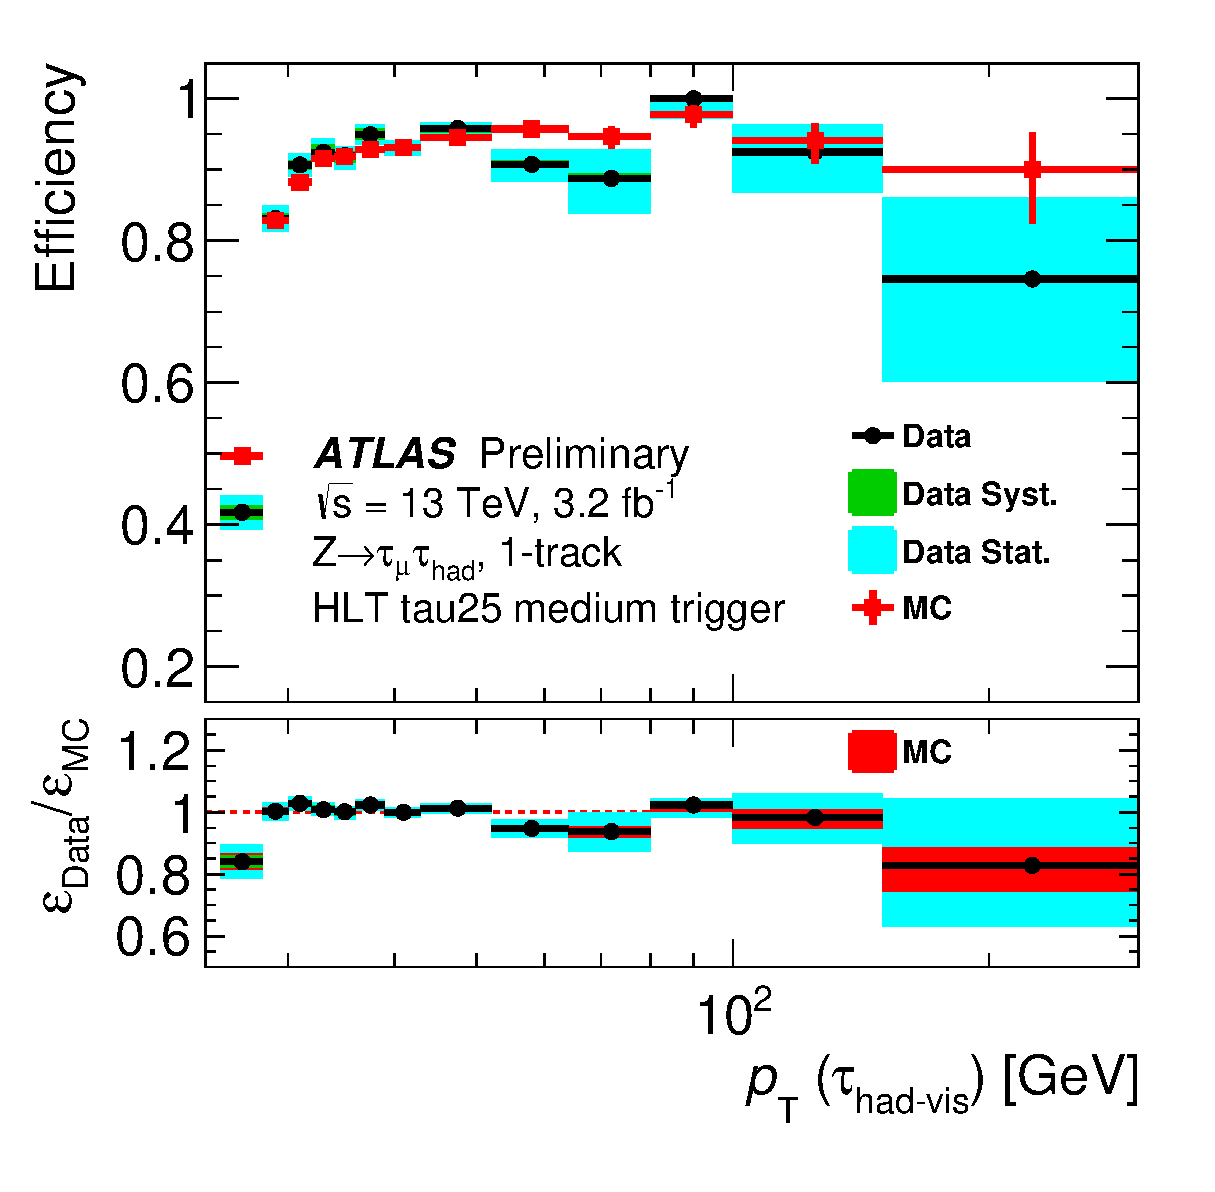
\includegraphics[width=0.45\textwidth]{./figures/object_selection/tau_trig_eff_ztt_1p.eps}
        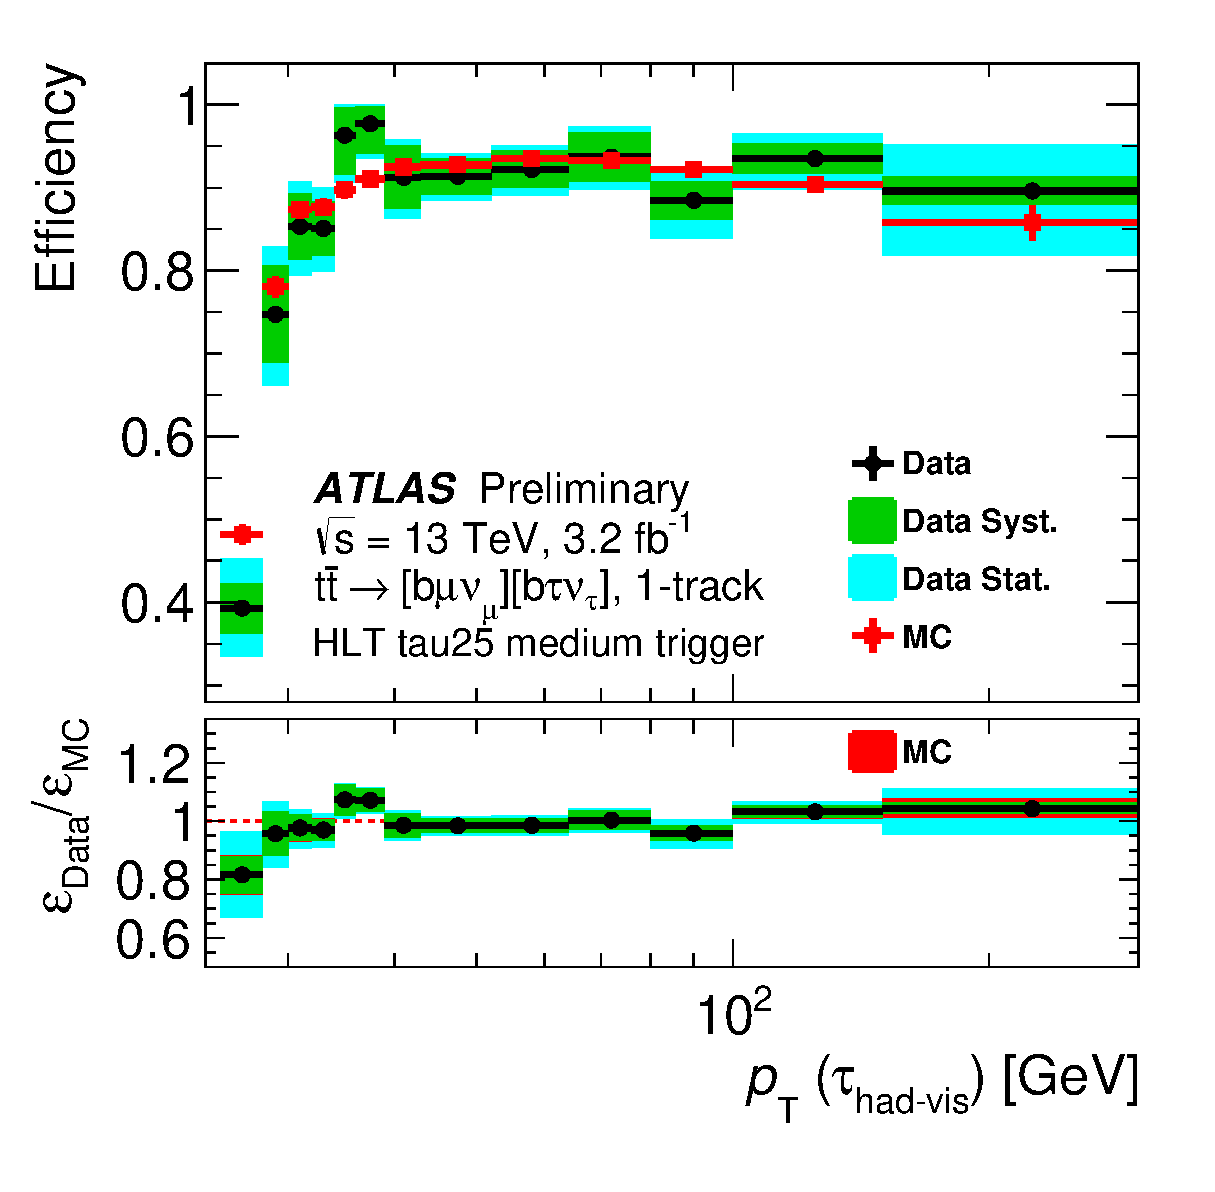
\includegraphics[width=0.45\textwidth]{./figures/object_selection/tau_trig_eff_tt_1p.eps}
        \caption{Tau trigger efficiencies and scale factors ($\epsilon_\text{Data} / \epsilon_\text{MC}$) for 1-pronged
        hadronic $\tau$ decays, measured in $\Z \to \tau\tau$ (left) and $\ttbar$ (right) events with
        the 2015 dataset.~\cite{ATLAS-CONF-2017-029}}\label{fig:object_selection:tau_eff}
    \end{center}
\end{figure}


\section{Missing Transverse Energy}\label{sec:object_selection:missing_transverse_energy}

In proton-proton collisions the exact momentum of the initial partons is not known.
However, the assumption can be made that partons carry no transverse momentum~\cite{PhysRev.185.1975}.
Thus, the transverse momentum in the final state should also be zero, due to energy and momentum conservation.
Any imbalance in the final state transverse momentum is known as the \emph{missing transverse energy} and denoted as \etmiss.
It arises from weakly-interacting, stable particles produced in the collision.
In the SM these particles are the neutrinos, but it may also be an indication of weakly-interacting exotic particles.
Since the focus of this analysis is the full leptonic decay $\Httllfull$, a large \etmiss{} contribution is expected
due to the four final state neutrinos.
Additional \emph{fake} \etmiss{} contributions can arise from pile-up or SM particles, which escape the detector without
being detected, are badly reconstructed, or cannot be reconstructed at all. These contributions distort the real \etmiss{}
and need to be corrected.

For the reconstruction of the missing transverse energy first the vectorial quantity \etmissvec{} is calculated
with reconstructed and calibrated physics objects~\cite{ATL-PHYS-PUB-2015-023}
\begin{equation}
    \label{eq:met:vector}
    \etmissvec = \etmissvecobj{e} + \etmissvecobj{\gamma} + \etmissvecobj{\tau} + \etmissvecobj{\text{jet}} + \etmissvecobj{\text{soft}} + \etmissvecobj{\mu} \,,
\end{equation}
with the missing transverse energy $\etmissvecobj{\text{type}} = - \sum \ptvec^\text{type}$ for each type of object
($e$: electrons, $\gamma$: photons, $\tau$: $\tau$-leptons, jet: jets, soft: soft objects, $\mu$: muons).
The individual contributions will be explained in the next paragraphs.
Most of the time and also in this analysis the scalar missing transverse energy \etmiss{} is used,
\begin{equation}
    \label{eq:met:scalar}
    \etmiss{} = \norm{\etmissvec{}} = \sqrt{{\left(\etmissx\right)}^2 + {\left(\etmissy\right)}^2} \,.
\end{equation}

The objects which are taken for \etmissvecobj{e}, \etmissvecobj{\mu}, \etmissvecobj{\tau},
and \etmissvecobj{\text{jet}} are described in the sections above.
\todo{Are photons used for the MET calculation in this analysis?}
The contributions for \etmissvecobj{\text{soft}} originate from  ID tracks associated with the primary vertex of the
hard interaction, which are not used in the reconstruction of the other, high \pt{} objects.
This is implemented in the Track Soft Term (TST) algorithm~\cite{ATL-PHYS-PUB-2015-023}.

The performance of the \etmiss{} reconstruction can be measured in $\Z \to \mpmm$ and $\W^\pm \to e^\pm \nu$
events comparing data to simulation. Those two processes provide events where either a genuine \etmiss{} contribution
is expected or not.
\cref{fig:object_selection:etmiss} shows the performance and resolution measured in $\Z \to \mpmm$ events.

\begin{figure}[htb]
    \begin{center}
        \includegraphics[width=0.45\textwidth]{./figures/object_selection/etmiss_performance_tst_zmm.eps}
        \includegraphics[width=0.45\textwidth]{./figures/object_selection/etmiss_resolution_tst_zmm.eps}
        \caption{Distributions of TST \etmiss{} (left) and the TST $E^\text{miss}_x, E^\text{miss}_y$ resolution (right)
        in $\Z \to \mpmm$ events.~\cite{ATL-PHYS-PUB-2015-027}}\label{fig:object_selection:etmiss}
    \end{center}
\end{figure}

\section{Overlap Removal}\label{sec:object_selection:overlap_removal}

It is possible that one particle can pass the reconstruction and identification requirements of multiple objects.
To remove this kind of ambiguity from the analysis an overlap removal is applied.
If two ore more objects are reconstructed within a certain distance \dr{} in the $(\eta - \phi)$ plane, only one object is kept.
First jets are removed, then hadronic $\tau$-leptons, and finally electrons.
Muons are ordered highest and are not removed.
Depending on the object combination, a different \dr{} threshold is used:

\begin{enumerate}
    \item hadronic $\tau$-leptons
        \begin{itemize}
            \item remove jets within $\dr = 0.2$
        \end{itemize}
    \item electrons
        \begin{itemize}
            \item remove jets within $\dr = 0.4$
            \item remove hadronic $\tau$-leptons within $\dr = 0.2$
        \end{itemize}
    \item muons
        \begin{itemize}
            \item remove jets within $\dr = 0.4$
            \item remove hadronic $\tau$-leptons within $\dr = 0.2$
            \item remove electrons within $\dr = 0.2$
        \end{itemize}
\end{enumerate}

\chapter{Event Selecton}\label{cha:event_selecton}

\section{Preselection}\label{sec:preselection}

\section{Categorization}\label{sec:categorization}

\chapter{Optimization of the Multivariate Analysis}\label{cha:mva_strategy}

\section{Event Selection}\label{sec:event}

\section{$k$-fold Cross-Validation}\label{sec:_k_fold_cross_validation}

\section{Hyperparameters}\label{sec:hyperparameters}

\section{Input Variables}\label{sec:input_variables}

\chapter{Systematic Uncertainties}\label{cha:systematic_uncertainties}

\chapter{Statistical Analysis and Results}\label{cha:fit}

In this chapter the likelihood fit is introduced, which is used to determine the signal strength of the $\Httllfull$ process.
For the multivariate analysis (MVA) the shape of the BDT output is used as the final discriminant.
In the cut-based analysis (CBA) the $\mmc$ distribution is used.
Furthermore, a strategy to obtain an optimal binning for the distribution of the BDT output is discussed.
Finally, the fit results are presented and compared between MVA and CBA\@.

\section{Likelihood fit}

The likelihood fit is used to determine the signal strength $\mu$, which is the ratio of the measured (fitted) signal cross-section to the
Standard Model prediction of the cross-section of $\Httll$.
A value of $\mu = 0$ indicates the absence of signal, $\mu = 1$ corresponds to the case that the amount of signal matches with the SM prediction.
The fit is executed with the \texttt{HistFactory} tool~\cite{HistFactory} using the \texttt{RooStats}~\cite{RooStats} package and the \texttt{WSMaker}~\cite{WSMaker} script collection.

The fit is based on a binned likelihood function $\mathcal{L}$~\cite{FitATLAS}, which originates from the Poisson distribution,
\begin{equation}
    \mathcal{L}(\mu, \bm{\theta}) = \prod_{i=1}^{N_\text{bins}} = \frac{{\left(\mu s_i (\bm{\theta}) + b_i(\bm{\theta})\right)}^{n_i} e^{-(\mu s_i (\bm{\theta}) + b_i(\bm{\theta}))}}{n_i!} \,.
\end{equation}
The binned likelihood function gives the probability of finding $n$ data events in the bin $i$, where $s$ signal events and $b$ background events are expected.
Here, the bins are not limited to one observable, but different contributions, for example single bin categories and binned distributions, can be combined in the likelihood.
Additionally, the likelihood function depends on several unknown parameters, $\bm{\theta} = (\theta_1, \ldots, \theta_m)$, which are discussed below.
A large value of the likelihood function indicates a better agreement between prediction and data.

The best fit value for $\mu$ is obtained by maximizing the likelihood function, and is denoted as $\hat{\mu}$.
However, it is more convenient to minimize the negative logarithm of the likelihood function, $- \ln \mathcal{L}$, which is also known as the negative log-likelihood (NLL).
Since the natural logarithm is a monotonically increasing function, this transformation can be made.
The log-likelihood transforms the product of the contributions of the individual bins in the normal likelihood function into a sum.
Due to the fact, that there are more advanced methods to minimize a function than finding its maximum, the negative sign is introduced.

In the search of new physics the compatibility between the observed data and the background-only hypothesis is an important quantity.
Therefore, the null hypothesis is $\mu = 0$ which needs to be rejected for an observation of the signal process.
For this analysis, a modified frequentist method known as $\text{CL}_s$~\cite{CLs} is used.

First, a test statistic $q_0$ is constructed~\cite{FitATLAS},
\begin{equation}
    q_0 =
    \begin{cases}
        -2 \ln (\mathcal{L}(0, \hat{\hat{\bm{\theta}}}) / \mathcal{L}(\hat{\mu}, \hat{\theta})) & \hat{\mu} \geq 0 \\
        0 &  \hat{\mu} < 0
    \end{cases} \,,
\end{equation}
where $\mathcal{L}(\hat{\mu}, \hat{\theta})$ refers to the maximum of the likelihood function and $\mathcal{L}(0, \hat{\hat{\bm{\theta}}})$ to
an conditional maximum where $\mu$ is fixed according to the null hypothesis.
The test statistic should have a good separation between the null hypothesis and the alternative hypothesis, where the signal strength is non-vanishing.
Using the probability density function of the test statistic, $g(q_0 | 0, \hat{\hat{\bm{\theta}}})$,
the compatibility of the null hypothesis with the observed test statistic $q_{0,\text{obs}}$
can be calculated, which is expressed with the $p_0$ value,
\begin{equation}
    p_0 = \int_{q_0,\text{obs}}^{\infty} g(q_0 | 0, \hat{\hat{\bm{\theta}}}) \dif q_0 \,.
\end{equation}
The $p_0$ value is the probability that the observed test statistic $q_{0,\text{obs}}$ is more compatible than the test statistic $q_0$ under
the null hypothesis.
If a negative amount of signal events is observed, which is unphysical, the test statistic is set to zero, since a positive amount is expected.

Usually the $p_0$-value is expressed in terms of Gaussian standard deviations.
This is the so-called \emph{significance} $Z_0$, which can be calculated by
\begin{equation}
    \label{eq:fit:significance}
    Z_0 = \Phi^{-1} (1 - p_0) \simeq \sqrt{q_0} \,.
\end{equation}
Here, $\Phi$ is the cumulative distribution function of the Gaussian distribution.
The asymptotic approximation~\cite{FitATLAS} is used in \cref{eq:fit:significance} to simplify the calculation.

An observation is claimed for a $p_0$-value of $p_0 < \num{10.5e-7}$, which corresponds to a significance of $Z_0 \geq 5$.

\section{Fitting Procedure}\label{sec:fit:procedure}

For the construction of the likelihood function several signal and control regions are used, which are discussed below.

In the cut-based analysis four signal regions, two for the VBF category and two for the boosted category as explained in \cref{sec:event_selection:categorization} is used.
The binning in setup in such a ways that there is at least some amount of background in each bin.
Under and overflow bins are included in the first and last bin, respectively.

An overview of the binning is given in \cref{tab:fit:regions:cba}.
To obtain the normalization of the $\Zll$and top-background a dedicated control region is used for each background.
There are separate control regions for the VBF and boosted category.
The definitions of the control regions can be found in \cref{sec:background_estimation:normalization}.
Since the control regions are used only for normalization purposes, only a single bin is used, which contains the complete event count.

\begin{table}[htpb]
    \centering
    \caption{Overview of the binning in the signal regions (SR) and control regions (CR) used in the fit for the cut-based analysis.}\label{tab:fit:regions:cba}
    \begin{tabular}{lcc}
        \toprule
        Region                              & Type  & Binning [GeV] \\ \midrule
        high VBF                            & SR    & $\left[60, 88, 116, 130, 200\right]$ \\
        low VBF                             & SR    & $\left[60, 88, 116, 130, 200\right]$ \\
        high boosted                        & SR    & $\left[60, 80, 110, 120, 130, 140, 200\right]$ \\
        low boosted                         & SR    & $\left[60, 80, 110, 120, 130, 140, 200\right]$ \\
        $\Zll$ VBF control region (CBA)     & CR    & single bin\\
        Top VBF control region (CBA)        & CR    & single bin\\
        $\Zll$ boosted control region (CBA) & CR    & single bin\\
        Top boosted control region (CBA)    & CR    & single bin\\
    \end{tabular}
\end{table}

In the multivariate analysis a similar approach is applied.
For the signal regions distributions of the BDT output after the modified event selection (\cref{sec:mva:event_selection}) are used.
In the boosted category the individual BDTs for same flavour (SF) and different flavour (DF) events are taken.
However, it turned out that splitting the events into SF and DF in the VBF category actually decreased the significance, because
insufficient amount of statistics.
Therefore, the BDTs for SF and DF events are combined by adding up the event yields in the individual bins.
The control regions are based on the modified event selection, but no other changes were made.

The binning for the BDT distributions is calculated with a method similar to the one used
in the Run-1 analysis of the $\Httlh$ channel~\cite{RuthmannPhd}.
Most signal events can be found at higher values of the BDT output distribution, whereas most background events
are located at low values.
A fine binning would allow for a better measurement of the signal strength, since bins in the region of high BDT values
would contain only a small number of background events.
However, each bin must contain at least some amount of background events to ensure that statistical fluctuations of the
background do not lead to empty bins.
The following algorithm provides the finest binning possible without violating the robustness of the background estimation.
A fine binned BDT distribution with 200 bins is used as an input.

Starting from the very signal like end of the BDT distribution the bins are merged if all of the following criteria are met:
\begin{itemize}
    \item The expected yield of the total background has to be larger than the expected yield of total background events in the current bin.
    \item The relative statistical uncertainty of each background ($\Zll$, $\Ztautau$, diboson, top, fake, $H \to WW$) has to be smaller than \SI{100}{\percent}.
    \item Either the expected yield yield of the total background is \SI{50}{\percent} larger than in the previous bin or
        the signal-to-background ratio is at most \SI{10}{\percent} smaller than in the previous bin.
\end{itemize}

The first criterion ensures a background shape which is monotonically decreasing.
Due to the second criterion it is ensured that statistical fluctuations of the background do not lead to empty bins.
The third criterion is used to create a new bin, if the bin offers higher signal sensitivity or if the background composition
is much different than in the previous bin.

The algorithm is applied on the BDTs for SF and DF events in the boosted category and on the combined BDT in the VBF category.
An overview of the different regions and binnings used in the multivariate analysis is shown in \cref{tab:fit:regions:mva}.

\begin{sidewaystable}[htpb]
    \centering
    \caption{Overview of the binning in the signal regions (SR) and control regions (CR) used in the fit for the multivariate analysis.}\label{tab:fit:regions:mva}
    \begin{tabular}{lcc}
        \toprule
        Region                              & Type  & Binning \\ \midrule
        VBF                                 & SR    & $\left[-1, -0.47, -0.24,  0.19, 0.59, 0.74, 1\right]$ \\
        Boosted SF                          & SR    & $\left[-1, -0.78, -0.44, -0.19, 0.12, 0.29, 0.41, 0.49, 0.57, 0.64, 0.69, 0.72, 1\right]$ \\
        Boosted DF                          & SR    & $\left[-1, -0.78, -0.5,  -0.21, 0.1,  0.31, 0.42, 0.5,  0.57, 0.61, 0.65, 0.67, 0.69, 1\right]$ \\
        $\Zll$ VBF control region (MVA)     & CR    & single bin\\
        Top VBF control region (MVA)        & CR    & single bin\\
        $\Zll$ boosted control region (MVA) & CR    & single bin\\
        Top boosted control region (MVA)    & CR    & single bin\\
    \end{tabular}
\end{sidewaystable}

\section{Results}\label{sec:fit:results}

The likelihood fit is carried out for both the cut-based and multivariate analysis.
Because this analysis is still under development and not yet approved by the ATLAS collaboration, the fit cannot be done
with the observed data.
Instead, the so-called \emph{Asimov data}~\cite{FitATLAS} is used, where the simulated events act as an replacement for the observed data.
However, the uncertainties are for the Asimov data are assumed to follow the Poisson distribution.
Therefore, the signal strength will be always one.
But the fit can still be used to obtain an expected sensitvity and to validate the fitting procedure.
The distributions of $\mmc$ which are used in the fit of the CBA are shown in \cref{fig:fit:input:cba:SR,fig:fit:input:cba:CR}, whereas the
corresponding distributions of the BDT output for the MVA are shown in \cref{fig:fit:input:mva:SR,fig:fit:input:mva:CR}.
As can be seen the control regions are relatively pure in their respectively processes.
The contributions of the ``fake'' background in the $\Zll$ control regions are minimal and therefore neglected.

\begin{figure}[htb]
    \centering
    \begin{subfigure}[t]{0.45\textwidth}
        \includegraphics[width=\textwidth]{./plots/fit/cba/sig_boostloose.pdf}
        \caption{low boosted}
    \end{subfigure}
    \begin{subfigure}[t]{0.45\textwidth}
        \includegraphics[width=\textwidth]{./plots/fit/cba/sig_boosttight.pdf}
        \caption{high boosted}
    \end{subfigure}
    \begin{subfigure}[t]{0.45\textwidth}
        \includegraphics[width=\textwidth]{./plots/fit/cba/sig_vbfloose.pdf}
        \caption{low VBF}
    \end{subfigure}
    \begin{subfigure}[t]{0.45\textwidth}
        \includegraphics[width=\textwidth]{./plots/fit/cba/sig_vbftight.pdf}
        \caption{high VBF}
    \end{subfigure}
    \caption{Distributions of $\mmc$ in the different signal regions with the binning used in the fit of the cut-based analysis.
             For the data shown in the plot Asimov data corresponding to the 2015 and 2016 dataset with $\SI{36.1}{\invfb}$ is used.}\label{fig:fit:input:cba:SR}
\end{figure}

\begin{figure}[htb]
    \centering
    \begin{subfigure}[t]{0.45\textwidth}
        \includegraphics[width=\textwidth]{./plots/fit/cba/zll_boost.pdf}
        \caption{$\Zll$ boosted}
    \end{subfigure}
    \begin{subfigure}[t]{0.45\textwidth}
        \includegraphics[width=\textwidth]{./plots/fit/cba/zll_vbf.pdf}
        \caption{$\Zll$ VBF}
    \end{subfigure}
    \begin{subfigure}[t]{0.45\textwidth}
        \includegraphics[width=\textwidth]{./plots/fit/cba/top_boost.pdf}
        \caption{Top boosted}
    \end{subfigure}
    \begin{subfigure}[t]{0.45\textwidth}
        \includegraphics[width=\textwidth]{./plots/fit/cba/top_vbf.pdf}
        \caption{Top VBF}
    \end{subfigure}

    \caption{Distributions of $\mmc$ in the different control regions with the binning used in the fit of the cut-based analysis.
             For the data shown in the plot Asimov data corresponding to the 2015 and 2016 dataset with $\SI{36.1}{\invfb}$ is used.}\label{fig:fit:input:cba:CR}
\end{figure}


\begin{figure}[htb]
    \centering
    \begin{subfigure}[t]{0.45\textwidth}
        \includegraphics[width=\textwidth]{./plots/fit/mva/sig_boostsf.pdf}
        \caption{Boosted SF}
    \end{subfigure}
    \begin{subfigure}[t]{0.45\textwidth}
        \includegraphics[width=\textwidth]{./plots/fit/mva/sig_boostdf.pdf}
        \caption{Boosted DF}
    \end{subfigure}
    \begin{subfigure}[t]{0.45\textwidth}
        \includegraphics[width=\textwidth]{./plots/fit/mva/sig_vbf.pdf}
        \caption{VBF}
    \end{subfigure}
    \caption{Distributions of the BDT output in the different signal regions with the binning used in the fit of the multivariate analysis.
             For the data shown in the plot Asimov data corresponding to the 2015 and 2016 dataset with $\SI{36.1}{\invfb}$ is used.}\label{fig:fit:input:mva:SR}
\end{figure}

\begin{figure}[htb]
    \centering
    \begin{subfigure}[t]{0.45\textwidth}
        \includegraphics[width=\textwidth]{./plots/fit/mva/zll_boost.pdf}
        \caption{$\Zll$ boosted}
    \end{subfigure}
    \begin{subfigure}[t]{0.45\textwidth}
        \includegraphics[width=\textwidth]{./plots/fit/mva/zll_vbf.pdf}
        \caption{$\Zll$ VBF}
    \end{subfigure}
    \begin{subfigure}[t]{0.45\textwidth}
        \includegraphics[width=\textwidth]{./plots/fit/mva/top_boost.pdf}
        \caption{Top boosted}
    \end{subfigure}
    \begin{subfigure}[t]{0.45\textwidth}
        \includegraphics[width=\textwidth]{./plots/fit/mva/top_vbf.pdf}
        \caption{Top VBF}
    \end{subfigure}
    \caption{Distributions of the BDT output in the different control regions with the binning used in the fit of the multivariate analysis.
             For the data shown in the plot Asimov data corresponding to the 2015 and 2016 dataset with $\SI{36.1}{\invfb}$ is used.}\label{fig:fit:input:mva:CR}
\end{figure}

The expected sensitivities for the cut-based and multivariate analysis are shown for fits done in the individual signal regions
and for the combination of all signal regions in \cref{tab:fit:result:sigma}.
The multivariate analysis manages to increase the sensitivity by approximately \SI{33}{\percent} and \SI{72}{\percent} in the boosted and VBF category, respectively.
For the combined fit of the boosted and VBF category the increase is about \SI{63}{\percent}.

\begin{table}[htpb]
    \centering
    \caption{Expected sensitivity for the cut-based (CBA) and multivariate (MVA) analysis of $\Httll$ for the combined and individual categories in units of $\sigma$.}\label{tab:fit:result:sigma}
    \begin{tabular}{lccccc}
        \toprule
        Analysis & Combined & Boosted & Boosted SF & Boosted DF & {VBF} \\ \midrule
        CBA      & 0.83     & 0.58    & --         & --         & 0.54  \\
        MVA      & 1.35     & 0.77    & 0.51       & 0.59       & 0.93  \\
        \bottomrule
    \end{tabular}
\end{table}

The results of the signal strength measurement in the cut-base and multivariate analysis are
\begin{align}
    \mu_\text{CBA} &= 1.0\, \errud{0.47}{0.46} \text{ (stat.) } \errud{1.25}{1.12} \text{ (sys.) }  \qquad \text{and} \\
    \mu_\text{MVA} &= 1.0\, \errud{0.32}{0.31} \text{ (stat.) } \errud{0.55}{0.66} \text{ (sys.) }  \,,
\end{align}
respectively.
Additionally, the results are visualized in \cref{fig:fit:result:mu}, where also the individual results for the VBF and boosted category are shown.
Since Asimov data is used in the fit, the expected values are 1.
However, it can be seen, that both the statistic and systematic uncertainties on the signal strengths are lower in the MVA than in the CBA\@.
In the VBF category the uncertainties are reduced by a factor between 1.5 and 3, which is the largest reduction for all signal strengths.
But signal strength of the combined fit and measurement in the boosted category the uncertainties are reduced by a factor of up to two.


\begin{figure}[htb]
    \centering
    \begin{subfigure}[t]{0.45\textwidth}
        \includegraphics[width=\textwidth]{./plots/fit/cba/POI.pdf}
        \caption{CBA}
    \end{subfigure}
    \begin{subfigure}[t]{0.45\textwidth}
        \includegraphics[width=\textwidth]{./plots/fit/mva/POI.pdf}
        \caption{MVA}
    \end{subfigure}
    \caption{Uncertainties on the signal strength measured in the of the cut-based analysis (a) and multivariate analysis (b)
             with Asimov data corresponding to the 2015 and 2016 dataset with $\SI{36.1}{\invfb}$.}\label{fig:fit:result:mu}
\end{figure}

A breakdown of the individual contributions to the uncertainties are given in \cref{tab:fit:result:uncert}.
The most dominat sources of uncertainty are related to measurements of jets and the missing transverse energy.
Furthermore, uncertainties due to simulation statistics and normalization are also major sources of uncertainty.

\begin{table}[htpb]
    \centering
    \caption{Uncertainty on the signal strength measurement in the cut-based (CBA) and multivariate (MVA) analysis
             with Asimov data corresponding to the 2015 and 2016 dataset with $\SI{36.1}{\invfb}$.}\label{tab:fit:result:uncert}
    \begin{tabular}{lcc}
        \toprule
         \multirow{2}{*}{Set of nuisance parameters} & \multicolumn{2}{c}{Impact on error}  \\
                                        & CBA        & MVA        \\ \midrule
         Total                          & $\pm 1.27$ & $\pm 0.68$ \\
         Data statistics                & $\pm 0.46$ & $\pm 0.32$ \\
         Systematic uncertainties       & $\pm 1.18$ & $\pm 0.60$ \\ \cmidrule{1-3}
         Normalization uncertainties    & $\pm 0.62$ & $\pm 0.25$ \\
         Jets and $\etmiss$             & $\pm 0.92$ & $\pm 0.45$ \\
         $b$-jets                       & $\pm 0.21$ & $\pm 0.03$ \\
         Light leptons                  & $\pm 0.12$ & $\pm 0.18$ \\
         Pileup reweighting             & $\pm 0.11$ & $\pm 0.04$ \\
         Fake estimation                & $\pm 0.17$ & $\pm 0.04$ \\
         Luminosity                     & $\pm 0.04$ & $\pm 0.04$ \\
         Theory unc.\ on signal         & $\pm 0.21$ & $\pm 0.09$ \\
         Theory unc.\ on $Z\to\tau\tau$ & $\pm 0.19$ & $\pm 0.07$ \\
         Simulation statistics          & $\pm 0.59$ & $\pm 0.32$ \\
         \bottomrule
    \end{tabular}
\end{table}

\chapter{Conclusion and Outlook}\label{cha:conclusion}


\appendix

\clearpage

\thispagestyle{plain}
\bibliographystyle{atlasBibStyleWithTitle}
\bibliography{bib}

\printindex%
\printglossaries%

\end{document}
